\section{Koblingsagent}
Ordet agent kommer av det latinske ordet ``agere'' som betyr å ``gjøre'' (Online Etymology dictionary, 2014)\citep{website:agent}. Betydningen beskriver i grove trekk en av agentenes viktigste funksjoner, nemlig å gjennomføre spesifikke oppgaver. Når det dreier seg om en mer teoretisk definisjon av en agent, og i denne forbindelse en software-agent, blir det mer problematisk. Det finnes mye litteratur om agenter og nesten like mange definisjoner. Nedenfor vil noen av disse definisjonene bli presentert.

\textit{``An autonomous agent is a system situated within and a part of an environment
that senses that environment and acts on it, over time, in pursuit of its own agenda
and so as to effect what it senses in the future''} \citep{agent}.

\textit{``An agent is an instantiation of an object together with an associated goal or a set of goals''} (Luck and D'Inverno, 1995)\citep{luck_dinverno_agent}.

\textit{``A software agent is a persistent, goal-oriented computer program that reacts to its environment and runs without continuous direct supervision to perform some function for an end user or another program''} (Gibilisco, 2013) \citep{website:gibilesco_agent}.

\textit{``Intelligent agents are software entities that carry out some set of operations on behalf of a user or another program with some degree of independence or autonomy, and in so doing,
employ some knowledge or representation of the user's goals or desires''} (Franklin \& Graesser, 1997)\citep{agent}

Schermer (2007)\citep{schermer} påstår at det verken finnes en felles definisjon eller felles definerte attributter for software-agenter. I stedet foreslås det at software-agenter kan ses på som en samlebetegnelse for softwareprogrammer som til en viss grad viser attributter som typisk assosieres med en agents funksjoner (Schermer, 2007)\citep{schermer}.

Til tross for at det er vanskelig å oppnå en felles definisjon av en agent, viser det seg at det ofte er en del karakteristikker som går igjen i agentbeskrivelser:
\begin{itemize}
\item Reaktiv
\item Proaktiv
\item Målorientert
\item Kommuniserende
\item Mobil
\item Fleksibel
\end{itemize}

(Franklin and Graesser, 1997)\citep{agent}, (Schermer, 2007)\citep{schermer}, (Nwana, 1996)\citep{nwana}

I fig. \ref{fig:agenter} illustreres de ulike typene av agenter som er foreslått av Franklin \& Graesser (1997)\citep{agent}. Ved bruk av denne kategoriseringen er det lettere å sette vår koblingsagent inn i kontekst. I og med at ``Gi bort dagens'' koblingsagent skal behandle data og gjøre beregninger ut i fra dette, går den inn under ``computational agents''. Videre kategoriseres koblingsagenten som en ``software agent''. Av de tre underkategoriene til ``software agents'' er det ``task-specific agent'' som er mest passende. Agenten har en spesifikk oppgave, nemlig å koble en mottaker med en giver basert på visse parametre. Noen av de viktigste karakteristikkene vår koblingsagent behøver for å kunne gjennomføre denne oppgaven er å være kommuniserende (må kommunisere med brukerne som er potensielle mottakere og givere), reaktiv (må reagere og aksjonere avhengig av hva brukerne fyller inn) og mobil (koblingsagenten må være tilgjengelig på alle enheter tilknyttet internett).


\begin{center}
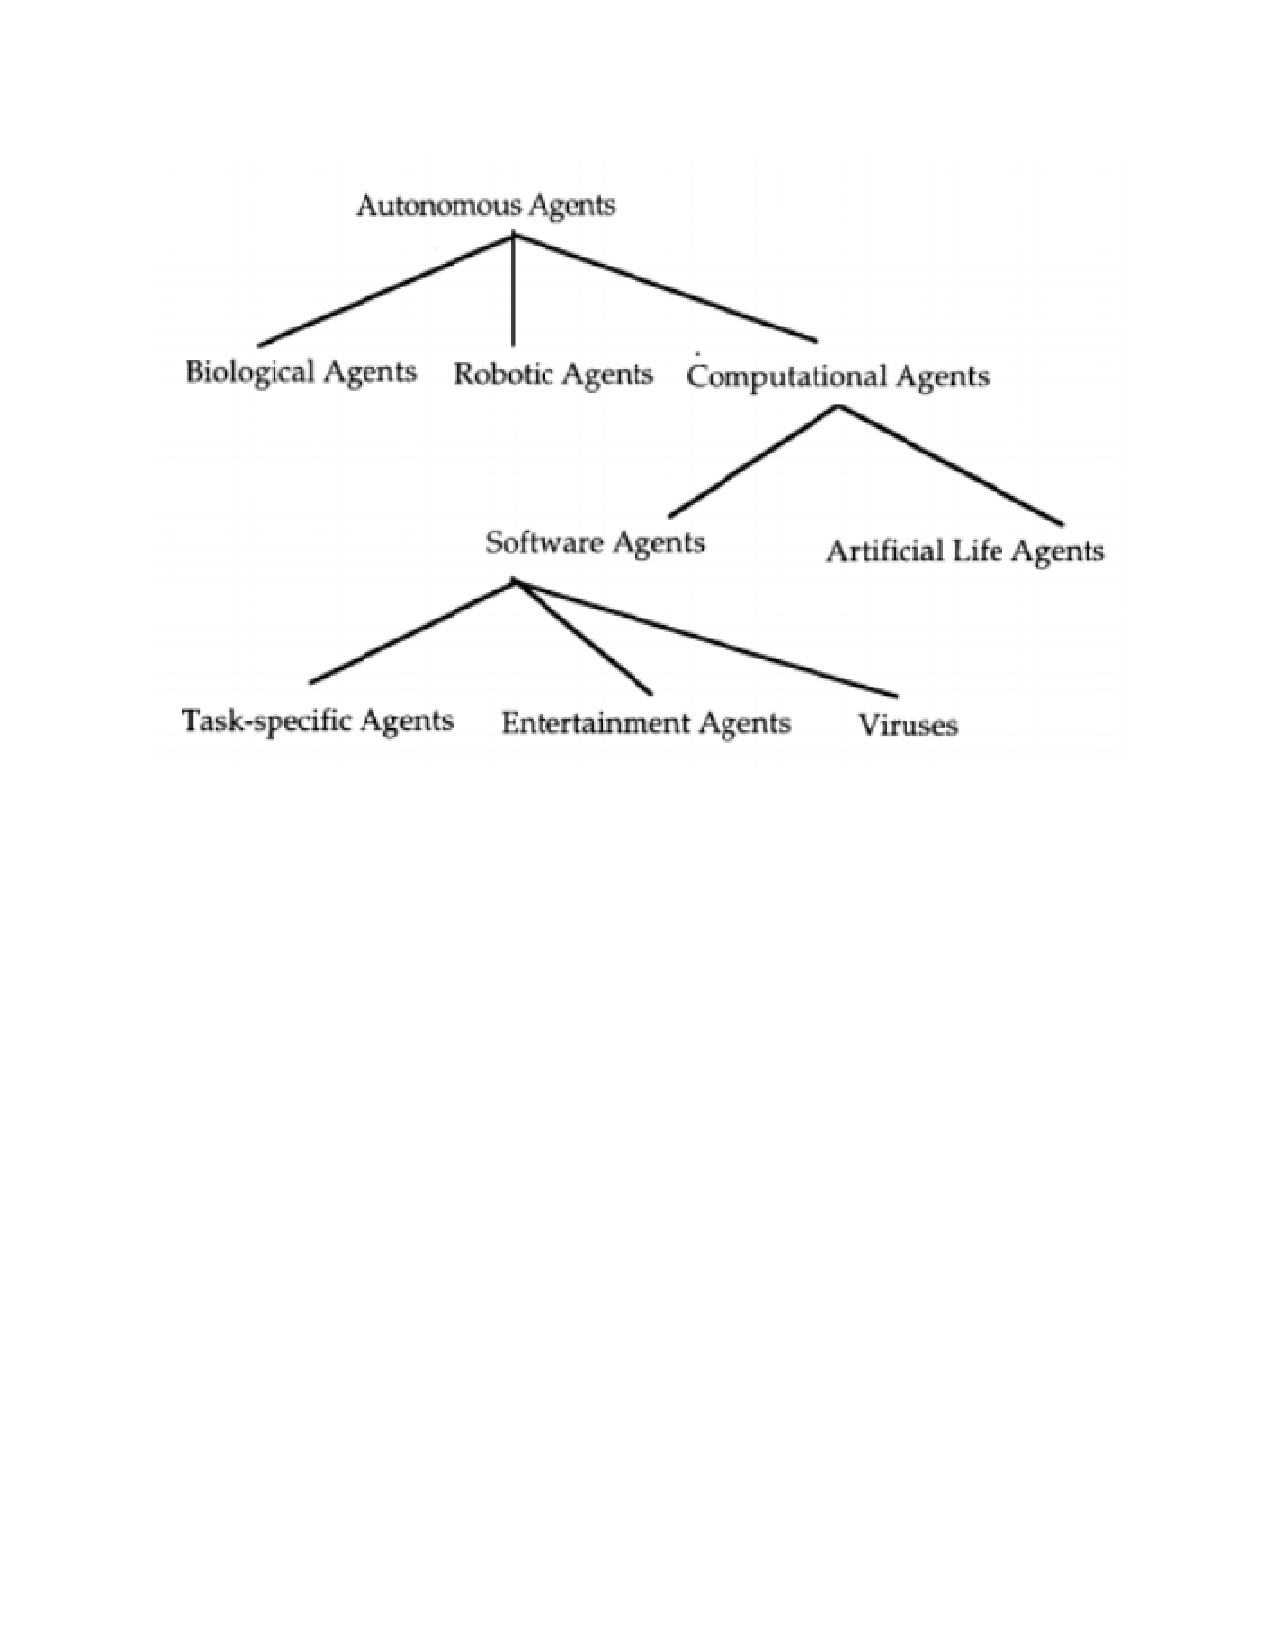
\includegraphics[clip=true, width=1 \textwidth,
trim=0cm 14cm 0cm 1.5cm]{agenter.pdf}
\captionof{figure}{Klassifiserting av ulike typer agenter}
\label{fig:agenter}
\end{center}
